	\documentclass[12pt,letterpaper,final]{report}
\usepackage[margin=2cm]{geometry}
\usepackage{setspace}
\usepackage{graphicx}
\usepackage{wrapfig}
\usepackage{caption}
\usepackage{subcaption}
\usepackage{amssymb}
\usepackage{gensymb}
\usepackage{amsmath}[fleqn]
\usepackage{lipsum}
\usepackage{cases}
\usepackage{chemist}
\usepackage{chemfig}
\usepackage[version=4]{mhchem}
\usepackage{chemmacros}
    \chemsetup{modules={all}}
\usepackage{lmodern}
\usepackage{textcomp}
\usepackage{placeins}
\usepackage{fancyhdr}

\usepackage{verbatim}
\usepackage{hyperref}
\usepackage{multicol}
\usepackage{multirow}
\usepackage{cancel}

\usepackage[style=apa,autolang=other, bibencoding =utf8,backend=biber,url=true,firstinits=true,language=auto,sorting=none]{biblatex}

\usepackage{tikz}
\usetikzlibrary{calc}

\usetikzlibrary{math}
\usetikzlibrary{angles,quotes}


\usepackage{tkz-euclide}
\usetikzlibrary{decorations.pathreplacing}
\usetikzlibrary{decorations.text}
\newcolumntype{P}[1]{>{\centering\arraybackslash}p{#1}}
\addbibresource{Sources.bib}


\begin{document}
\section{Scope}
Evaporation is a widespread phenomenon found in nature, but also very useful in food processing, chemical and other industries. As it is a time consuming process, the question of its prediction is essential when planning and organizing large scale production. This is also a very important problem for environmental sciences, especially the modeling of water cycles and their relation to global warming. Within both of these examples, the area of evaporation is a contributing factor to its rate.
\medskip
\\* The goal of this investigation is to establish and verify a mathematical model for the effect of evaporation surface area on the actual volume of evaporated liquid for the case of water.
\section{Research Question}
What is the effect of surface area (47.5, 47.1,57.3,29.5,90.6 \ce{cm^{2}}) on the volume of evaporated water as determined by measuring the change in water level due to evaporation over a duration of 724.95 hours at constant temperature of 297 K$\degree$ ?

\section{Background Information}
A large multi-particle system can be modeled by considering the probability of each particle being in a given state (\cite{stats}). For a system in constant conditions, these probabilities are assumed to be constant.

\medskip
\noindent Temperature of a system is the measure of the average kinetic energy of all of its particles. Units of degrees Kelvin are used for this definition, with the origin of the scale representing a stationary particle (no kinetic energy at all) and 1 K$\degree$ being equal in magnitude to 1 C$\degree$ (\cite{kelvin}).
\medskip
\\* All particles of the same compound are identical in size and mass, regardless of the state they are in. Gaseous particles however, have a higher kinetic energy (speed) than particles of a liquid (\cite{phase}). 
\medskip
\\* To evaporate, a particle must have sufficient energy to break the liquid's intermolecular bonds as well as be on its surface (\cite{evap}). 
\medskip
\\* The rate of evaporation can be affected by the saturation of liquid vapour in the air (\cite{evap}).
\medskip
\\* The area of a circle is calculated using the following equation (\cite{circle}):
\begin{equation} \label{eq:circa}
S = \pi \left(\frac{d}{2}\right)^{2}
\end{equation}
\medskip
\\* Where:
\medskip
\\* $S$ - area of the circle
\\* $d$ - diameter of the circle
\section{Hypothesis}
Consider an open-top container with straight edges, filled with some liquid and held at a constant temperature. 
\medskip
\\* Some minimum energy ($E_{ev}$) is required for a liquid molecule to be able to evaporate. Assuming the average temperature stays constant and the liquid is not in motion (conditions are constant), we can state the the probability of a particle being capable of evaporating is constant. For a large quantity of particles (macroscopic size liquid) we can then assume the total number of evaporation ready particles is constant.
\medskip
\\* We will assume that the liquid is equally mixed, with every unit of volume having the same quantity of molecules with energy greater than $E_{ev}$. 
\medskip
\\* Recall that particles can only evaporate at the very top of the liquid. Therefore the total volume of particles ready to evaporate is proportional to the surface area:
\medskip
\begin{equation}\label{eq:prop1}
V_{r} \propto  S 
\end{equation}
\medskip
\begin{wrapfigure}[12]{r}{1.8in}
\begin{center}
\vspace{-2 cm}
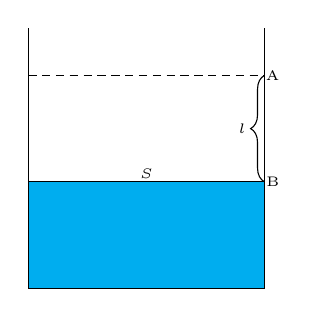
\begin{tikzpicture}[scale=3]


\coordinate (tl) at (0,1.4);

\coordinate (bl) at (0,0.3);

\coordinate (br) at (1,0.3);

\coordinate (tr) at (1,1.4);

\coordinate (topll) at (0,1.2);

\coordinate (toplr) at (1,1.2);

\coordinate (sndll) at (0,0.75);

\coordinate (sndlr) at (1,0.75);


\node[xshift = 3] (A) at (toplr) {\tiny A};

\node[xshift = 3] (B) at (sndlr) {\tiny B};


\fill[fill = cyan]  (sndll) rectangle (br);

\draw (tl)--(bl)--(br)--(tr);

\draw[densely dashed] (topll) -- (toplr);

\draw (sndll) -- (sndlr) node[midway, yshift = 3pt] {\tiny $S$};



%\draw [decorate,decoration= {brace,amplitude = 2pt},xshift=8  pt,yshift=0 pt]  ($ (topll)!0.5!(toplr) $)-- ($ (sndll)!0.5!(sndlr) $) node [midway,xshift=3 pt ]  {\tiny $l$};

\draw [decorate,decoration= {brace,amplitude = 5pt},xshift=8  pt,yshift=0 pt]  (sndlr)-- (toplr) node [midway,xshift=-8 pt ]  {\tiny $l$};

\end{tikzpicture}
\end{center} 
\caption{A - initial water level. B - new water level after some time $t$. $l$ - the position of the new water level relative to initial. $S$ - surface area of evaporating liquid}\label{fig:ev}
\end{wrapfigure}
\\* Where: 
\medskip
\\* $V_{r}$ - volume of liquid that can evaporate
\\* $S$ - surface area of liquid
\medskip
\\* Now let's consider the rate of evaporation to time. Assuming that the column of water is infinitely high (the decrease in water level over time, does not affect the process of evaporation), we can state that the liquid evaporates at a constant rate (as by our definition none of the relevant conditions change). We will also assume that the change in liquid concentration in the air due to evaporation, will not change the rate of evaporation significantly and can be ignored.
\medskip
\\* The volume of liquid evaporated over time, should therefore be proportional to time and the volume of evaporation ready particles. 
\medskip
\begin{equation}\label{eq:prop2}
V_{e} \propto V_{r}\cdot t 
\end{equation}
\\* Where:
\medskip
\\* $V_{e}$ - total volume of liquid evaporated after time $t$
\\* $V_{r}$ - volume of evaporation ready particles
\\* $t$ - time liquid has been left to evaporate for 
\medskip
\\* Substitute proportionality statement (\ref{eq:prop1}) into the equation above to get:
\medskip
\\* $$ V_{e} \propto S\cdot t$$
\medskip
\\* Using Figure (\ref{fig:ev}), we can rewrite the volume of evaporated liquid as:
\begin{equation}\label{eq:vol}
V_{e} = S\cdot l 
\end{equation}
\medskip
\\* Where:
\medskip
\\* $V_{e}$ - total volume of liquid evaporated
\\* $S$ - surface area of liquid
\\* $l$ - the decrease in surface level due to evaporated liquid (Figure  \ref{fig:ev})
\medskip
\\* Substitute \ref{eq:vol} into proportionality statement (\ref{eq:prop2}) and simplify to get:
\\* $$\cancel{S}\cdot l \propto \cancel{S}\cdot t $$
\begin{equation*}
l \propto t
\end{equation*}
\medskip
\\* Let's introduce some proportionality coefficient $k$ and rewrite the equation above as:
\begin{equation}\label{eq:hyp}
l = k\cdot t
\end{equation}
\medskip
\\* Where:
\\* $l$ - reduction in water level over time (Figure \ref{fig:ev})
\\* $k$ - some coefficient unique to the liquid, temperature and liquid vapour saturation
\\* $t$ - time elapsed since beginning of evaporation.
\medskip
\\* It is expected that the relationship in (\ref{eq:hyp}) will be held for the evaporation of water. Combined with equation (\ref{eq:vol}), surface area would therefore be proportional to the volume of liquid evaporated over time.
\section{Experiment}

\subsection{Materials and Equipment}
\subsubsection*{Equipment}
\begin{itemize}
\item 5 clear glass (or other material inert with water) cylindrical jars with straight edges (sides) and cross-sections of different area 

\item Permanent marker (or other writing utensil) that can be used on glass (or inert material of your choice)

\item Ruler ($\pm$ 0.1 cm)
\item Device that can measure long periods of time (over 730 hours) ($\pm$ 1 min)
\end{itemize}
\subsubsection*{Materials}
\begin{itemize}
\item Tap water (2 L)
\end{itemize}
\pagebreak
\subsection{Procedure}
\begin{wrapfigure}{R}{1.5in}
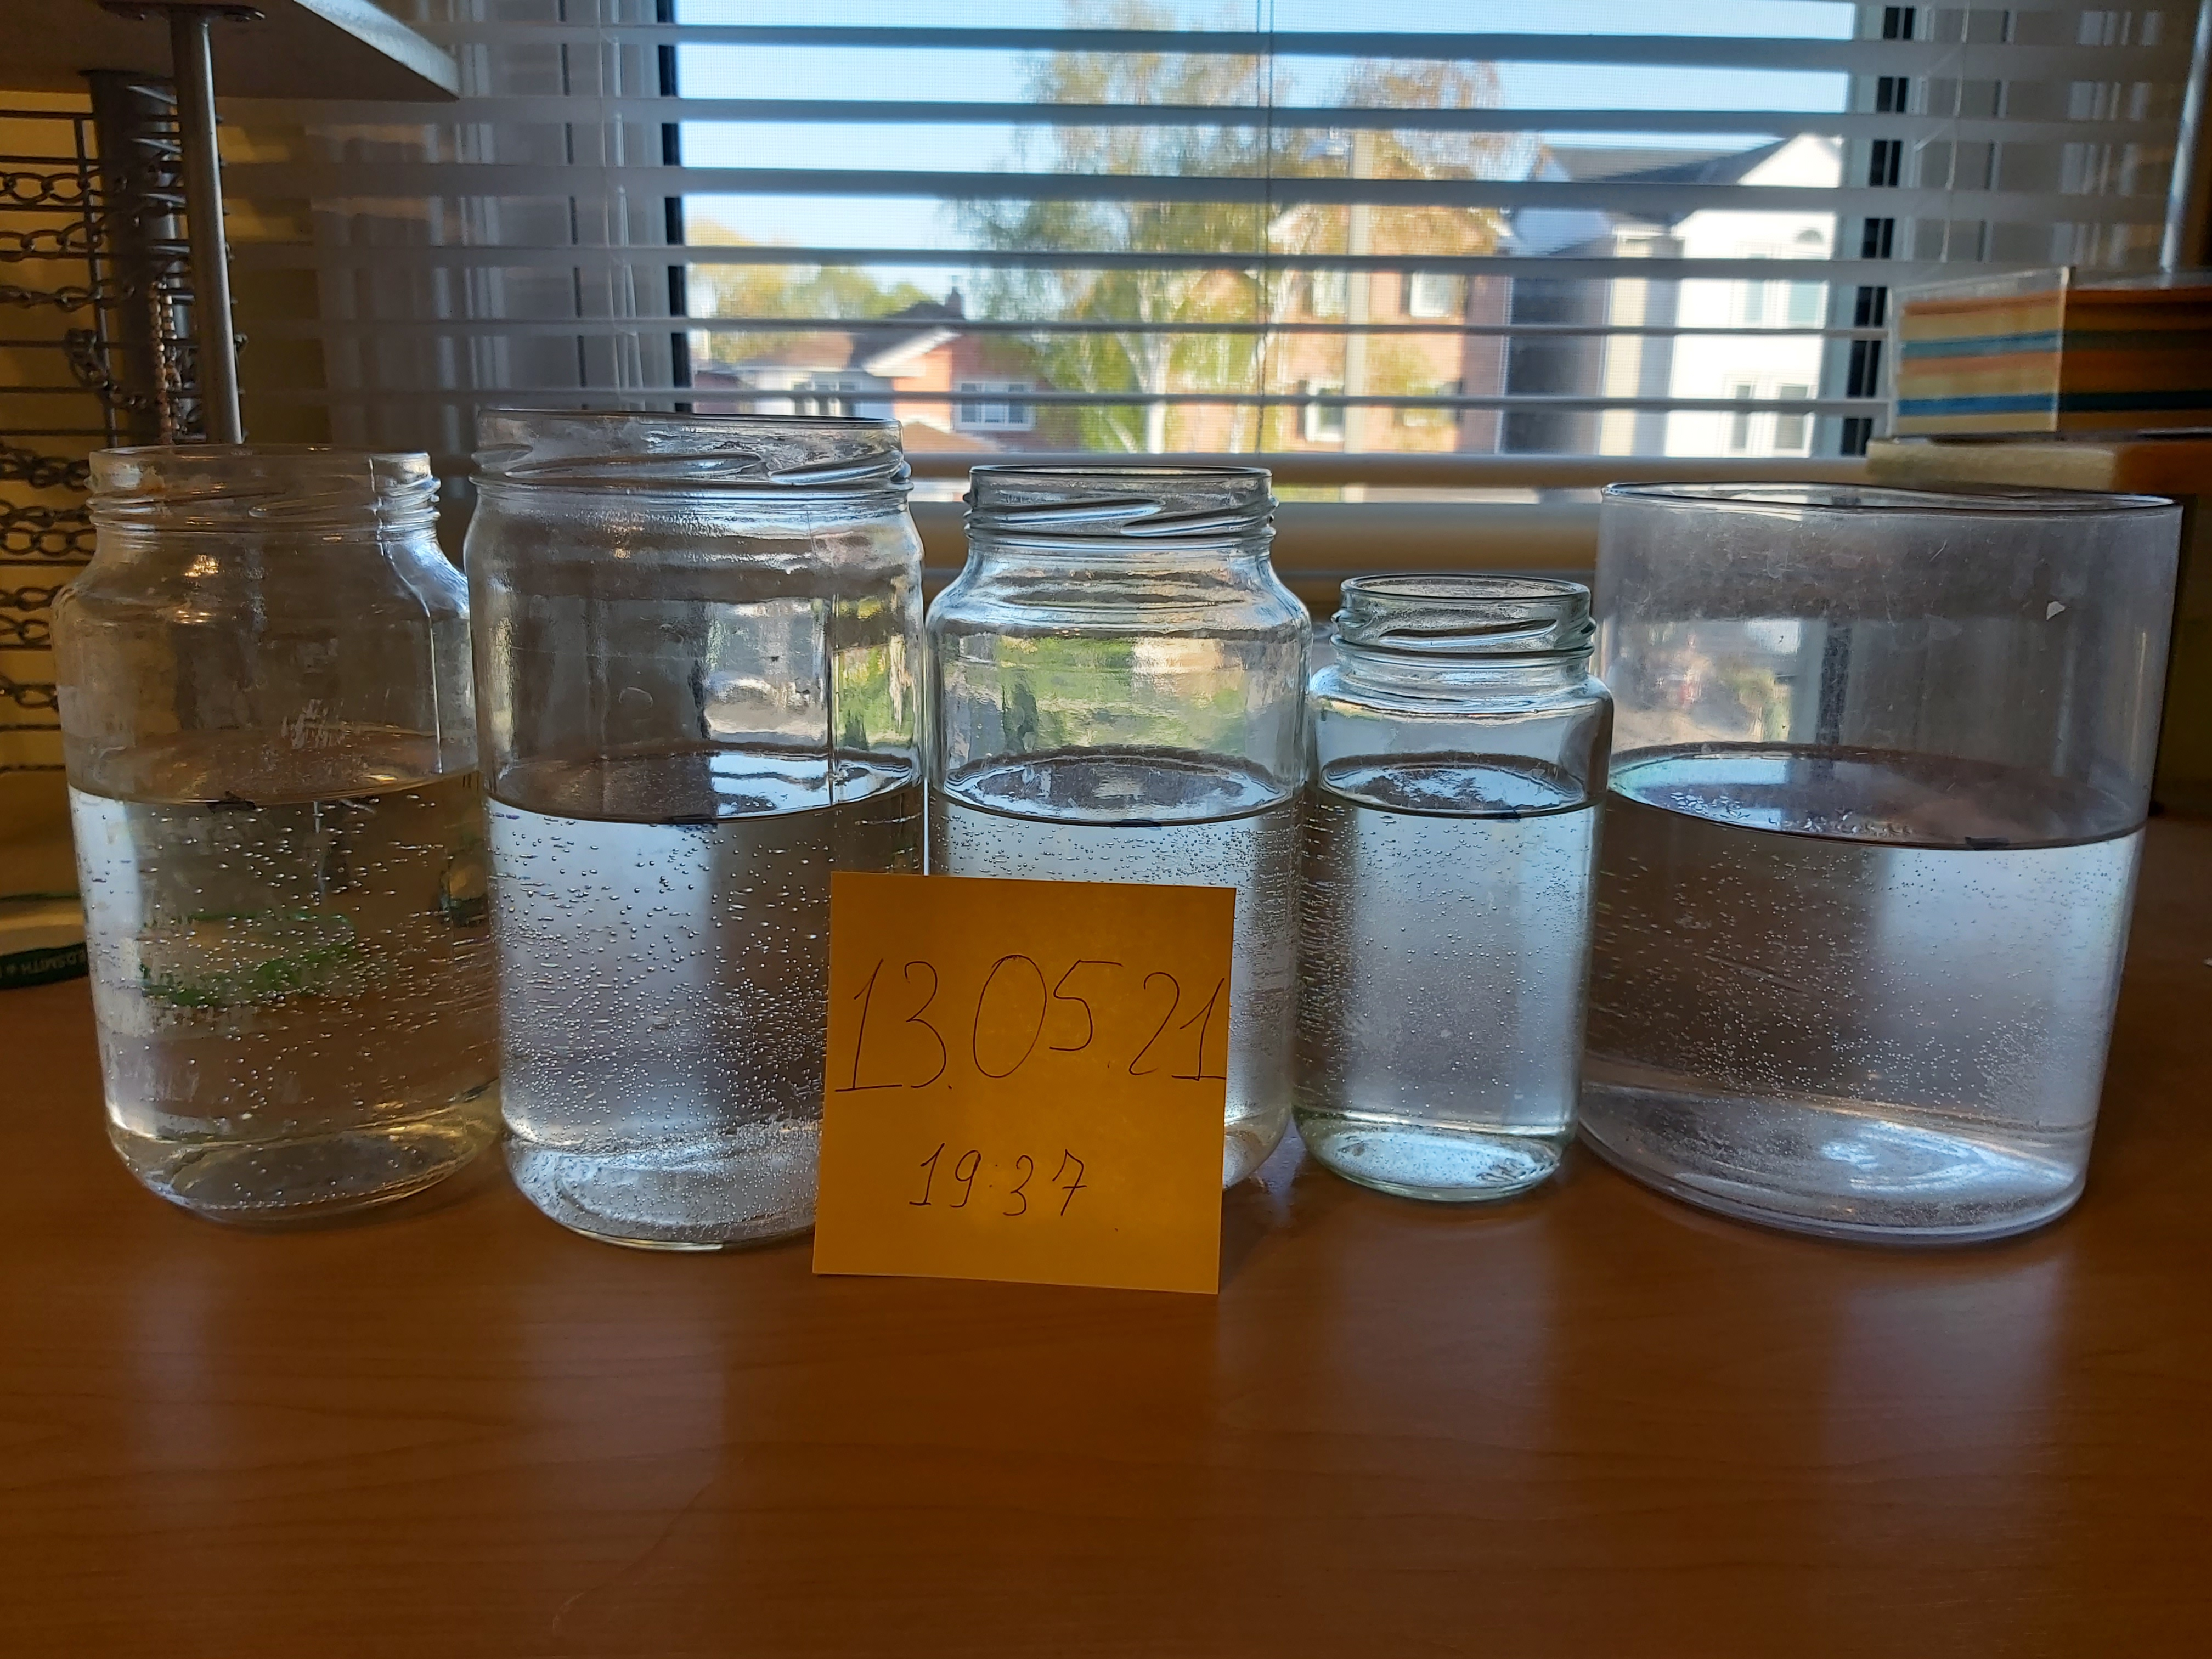
\includegraphics[width=0.2 \textwidth]{Jars1.jpg}
\caption{Cylindrical jars were filled to the same level. This water level was marked with a sharpie. Time of marking was recorded}
\end{wrapfigure}
The 5 clear jars dry jars, were filled with tap water upto 8.3 cm above their bottoms. This initial water level was marked on the jars. They were then left open (no lids) in a room, kept away from direct sunlight/any heating sources. Every 5-7 days the new water level was marked and its distance from the initial level and time of measurement were recorded. In total, 5 markings (disregarding the initial one) were made over the course of 30 days.


\subsection{Variables}
\begin{itemize}
\item Temperature of water ($T$)
\begin{itemize}
\item A change in the average temperature of the liquid will change the percentage of particles able to evaporate.
\item As all of the samples were placed in one room, and were therefore affected by changes in temperature in an identical fashion, and the water level $l$ will change identically for all jars.
\item The experiment proceeded at the current temperature of the room, with temperature ranging from 297 K$\degree$ to 300 K $\degree$. This is a very small relative change and the effect of temperature can be ignored. 
\end{itemize}
\item Surface area
\begin{itemize}
\item Surface area $S$ was kept constant within each sample by using jars with straight sides. 
\end{itemize}

\item Water vapour concentration in the air
\begin{itemize}
\item The jars were left in a large room. The volume of the room (3m $\times$ 4m $\times$ 5 m) is more than 100 times greater than than the 2 L volume of water. Effects of vapour concentration can therefore be considered to as negligible. 
\end{itemize}


\end{itemize}
\section{Data Analysis}
\subsection{Methodology}
In order to verify relationship (\ref{eq:hyp}), graphs of decrease in water level over time were constructed and proportionality coefficients $k$ were calculated for each jar. They were then compared for consistency between all samples.
\medskip
\\* Minimum and maximum possible proportionality coefficients (slopes) were calculated using the first and last points in each data set. They were then compared to the exact coefficient to determine its uncertainty.
\medskip
\\* Min/max slopes are calculated using the following formulas:
\begin{equation}\label{eq:min}
k_{min} = \frac{l_{1}-\delta l}{t_{1}+ \delta t}
\end{equation}
\begin{equation}\label{eq:max}
k_{max} = \frac{l_{1}+\delta l}{t_{1}-\delta t}
\end{equation}
\medskip
\\* Where:
\\* $l_{1}$ - overall change in water level in the experiment 
\\* $\delta l$ - uncertainty of water level change measurement
\\* $t_{1}$ - total time between marking of first and last point
\\* $\delta t$ - uncertainty of time measurements
\medskip
\\* *Note that as equation (\ref{eq:hyp}) implies a proportional relationship, the first point of the series is assumed to be exactly at (0;0).
\medskip
\\* The uncertainty for the proportionality coefficient is then calculated using:
\medskip
\begin{equation} \label{eq:unc}
\delta k = \max \left ( \left| k_{ex} - k_{min}\right|; \left | k_{ex}-k_{max}\right| \right )
\end{equation}
\subsection{Raw Data}
\FloatBarrier
\begin{table}[h!] 

\begin{center}
\caption{Decrease in water level over time due to evaporation, in 5 cylindrical jars of different diameter as measured over the course of 31 days at temperatures ranging from 297 K$\degree$ to 300 K$\degree$}
\begin{tabular}{|P{2.5cm}|P{2.5cm}|P{2.5cm}|P{2.5cm}|P{2.5cm}|P{2.7cm}|}
\hline
& Jar 1 \newline $d= \newline (7.78$ $\pm$ 0.01) cm & Jar 2 \newline $d= \newline (8.54$ $\pm$ 0.01) cm &Jar 3 \newline $d= \newline (7.75$ $\pm$ 0.01) cm & Jar 4 \newline $d= \newline (6.13$ $\pm$ 0.01) cm  & Sample 5 \newline $d= \newline (10.74$ $\pm$ 0.01) cm  \\ \hline
Time after initial marking \newline ($t$) ($\pm$ $\frac{1}{60}$ h)& \multicolumn{5}{P{12.7 cm}|}{\vspace{0.5cm} Distance away from initial water level after some time $t$ \newline ($l$) ($\pm$ 0.1 cm)} \\ \hline
0.00&	0.0 &	0.0 &	0.0 &	0.0 &	0.0 \\ \hline
119.43&	0.5	&0.7&	0.6&	0.6	& 1.0\\ \hline
236.15&	1.3&	1.4&	1.3&	1.3&	1.6\\ \hline
460.35&	2.5&	2.6	&2.3&	2.2&	2.6\\ \hline
592.65& 3.1&	3.2&	2.8	&2.8&	3.4\\ \hline
724.95&	3.7&	4.0&	3.5&	3.4&	4.1\\ \hline

\end{tabular}
\label{Tab:raw}
\end{center}
\end{table} \FloatBarrier

\subsection{Sample Calculations and Analysis}
Using Mathematica's fit function and data for Jar 1 in Table (\ref{Tab:raw}), find the proportionality coefficient $k_{1}$ to be:
\medskip
\\* $\displaystyle k_{1} = 0.0052$ \ce{\frac{cm}{h}}
\medskip
\\* Using  data from Table (\ref{Tab:raw}) equations (\ref{eq:min}) and (\ref{eq:max}), calculate the min max proportionality coefficients to be:
\medskip
\begin{flalign*}
k_{1min} & =  \frac{3.7-0.1}{724.95+ \frac{1}{60}}      &&
\\ &=0.0050 \, \, \ce{\frac{cm}{h}}
\end{flalign*}
\begin{flalign*}
k_{1max} & = \frac{3.7 + 0.1}{724.95 - \frac{1}{60}} &&
\\* &= 0.0052 \, \, \ce{\frac{cm}{h}}
\end{flalign*}
\medskip
\\* Using equation (\ref{eq:unc}) and minimum and maximum proportionality coefficients from above, calculate the uncertainty for the exact proportionality coefficient. 
\medskip
\begin{flalign*}
\delta k_{1} &= \max \left (\left |k_{1}-k_{1min}\right|; \left |k_{1}-k_{max} \right| \right)  &&
\\* &= \max \left (\left | 0.0052 - 0.0050 \right| ; \left | 0.0052-0.0052  \right| \right)
\\* &= 0.0002 \, \, \ce{\frac{cm}{h}}
\end{flalign*}
\medskip
\\* Calculate the surface area of the liquid using equation (\ref{eq:circa}) and the diameter of Jar 1 from (\ref{Tab:raw}), assuming that the cylinder has a perfectly circular face. 
\begin{flalign*}
S_{1} &= \pi \left (\frac{d}{2}\right )^{2} &&
\\* &= \pi \left ( \frac{7.78 \pm 0.01}{2} \right )^{2}
\\* &= (47.5 \pm 0.2) \ce{cm^{2}}
\end{flalign*}

\begin{figure}[h!]
\begin{center}
\includegraphics[width = 0.7\textwidth]{Graphs/G1.png}
\caption{Change in water level due to evaporation over time for Jar 1 with an evaporation surface area of (47.5 $\pm$ 0.1) \ce{cm^{2}} using data from Table (\ref{Tab:raw}).  Exact proportional fit - solid line; Maximum slope proportional fit - dash dotted line; Minimum slope proportional fit - dashed line. Proportional fit with a slope coefficient of $k_{1}$ =(0.0052 $\pm$ 0.0002) \ce{\frac{cm}{h}} and $R^{2}$ = 0.99} \label{fig:gr1}
\end{center}
\end{figure} \FloatBarrier
\medskip \noindent Similarly plot graphs for all other jars in Table (\ref{Tab:raw}):\FloatBarrier
\begin{figure}[h!]
\begin{center}
\begin{subfigure}[b]{0.48 \textwidth}
\includegraphics[width = 1\textwidth]{Graphs/G2.png}
\caption{Change in water level due to evaporation over time for Jar 2 with an evaporation surface area of (57.3 $\pm$ 0.1)  \ce{cm^{2}} using data from Table (\ref{Tab:raw}). Proportional fit with a slope coefficient of $k_{2}$ = (0.0055 $\pm$ 0.0002) \ce{\frac{cm}{h}} and $R^{2}$ = 0.99}
\end{subfigure}%%
\hfill
\begin{subfigure}[b]{0.48 \textwidth}
\includegraphics[width = 1\textwidth]{Graphs/G3.png}
\caption{Change in water level due to evaporation over time for Jar 3 with an evaporation surface area of (47.2 $\pm$ 0.1)  \ce{cm^{2}} using data from Table (\ref{Tab:raw}). Proportional fit with a slope coefficient of $k_{3}$ = (0.0049 $\pm$ 0.0002)  \ce{\frac{cm}{h}} and $R^{2}$ = 0.99}
\end{subfigure}%
 \hfill
\begin{subfigure}[b]{0.48 \textwidth}
\includegraphics[width = 1\textwidth]{Graphs/G4.png}
\caption{Change in water level due to evaporation over time for Jar 4 with an evaporation surface area of (29.5 $\pm$ 0.1)  \ce{cm^{2}} using data from Table (\ref{Tab:raw}). Proportional fit with a slope coefficient of $k_{4}$ = (0.0048 $\pm$ 0.0002)  \ce{\frac{cm}{h}} and $R^{2}$ = 0.99}
\end{subfigure}%
\hfill
\begin{subfigure}[b]{0.48 \textwidth}
\includegraphics[width = 1\textwidth]{Graphs/G5.png}
\caption{Change in water level due to evaporation over time for Jar 5 with an evaporation surface area of (90.6 $\pm$ 0.2)  \ce{cm^{2}} using data from Table (\ref{Tab:raw}). Proportional fit with a slope coefficient of $k_{5}$ = (0.0058 $\pm$ 0.0003)  \ce{\frac{cm}{h}} and $R^{2}$ = 0.99}
\end{subfigure}%
\caption{Proportional best fits for jars 2-5 using data from Table (\ref{Tab:raw}). Exact proportional fit - solid line; Maximum slope proportional fit - dash dotted line; Minimum slope proportional fit - dashed line } \label{fig:graphr}
\end{center}
\end{figure}\FloatBarrier
\noindent Calculate the average coefficient to be:
\medskip
\\* $k_{av} = (0.0052 \,\, \pm \,\, 0.0002 $) \ce{\frac{cm}{h}}
\medskip
\\* Using Mathematica's StandardDeviation function, calculate the normalized standard deviation:
\medskip
\\* $\displaystyle \sigma_{n} = 0.082$ 

\section{Conclusion}
The validity of the proposed relationship (\ref{eq:hyp}) was verified by comparing the change in water level due to evaporation over time between 5 samples with different evaporation surface areas. All jars showed a consistent fit with an average coefficient of $k_{av}=0.052$ and a relatively low standard deviation among samples was less than 10 \% of the actual value. This is further supported by high $R^{2}$ values of 0.99 among all jars.
\medskip
\\* Overall, this demonstrates equation (\ref{eq:hyp}) to be an accurate model for evaporation of water, strongly suggesting the initial assumption of a proportional effect of area on evaporation to be correct.


\section{Limitations and Extensions}
The samples showed a normalized deviation of around 8\% which prevents establishing a more exact $k$ coefficient to be used for accurate predictions. This could have been caused by the different bottle neck shape of the jars used (Figure \ref{fig:ev}). While they do not directly directly affect the water itself, they can create a point of congestion for the vapour, which would decrease the evaporation rate. This suggestion is consistent with the experimental results as jars 3 and 4, having the greatest relative decrease in area at the top of their opening also had the smallest $k$ coefficients and jar 5 with perfectly straight edges, had the greatest $k$ coefficient. This can be negated by using containers with straight sides in future experiments. Water vapour saturation can also be kept constant with consistent air ventilation over the top of the containers, and frequent confirmation measurements with a hydrogemeter.

\printbibliography[heading=subbibliography, title= Bibliography]

\end{document}